\documentclass[a4paper,10pt]{article}
\usepackage[utf8]{inputenc}
\usepackage{graphicx}
\usepackage{subcaption}
\usepackage{parskip}
\usepackage{amsmath}
\usepackage{listings}
\usepackage{color}
\usepackage{listings}

\definecolor{red}{rgb}{1,0,0}
\definecolor{green}{rgb}{0,1,0}
\definecolor{codegreen}{rgb}{0,0.6,0}
\definecolor{codegray}{rgb}{0.5,0.5,0.5}
\definecolor{codepurple}{rgb}{0.58,0,0.82}
\definecolor{backcolour}{rgb}{0.95,0.95,0.92}

\lstdefinestyle{mystyle}{
    backgroundcolor=\color{backcolour},   
    commentstyle=\color{blue},
    numberstyle=\tiny\color{codepurple},
    stringstyle=\color{codegreen},
    basicstyle=\footnotesize,
    breakatwhitespace=false,         
    breaklines=true,                 
    captionpos=b,                    
    keepspaces=true,                 
    numbers=left,                    
    numbersep=5pt,                  
    showspaces=false,                
    showstringspaces=false,
    showtabs=false,                  
    tabsize=2
}
 
\lstset{style=mystyle,language = C}

%opening
\title{LIC, UNIK4660 Obligatory Assignment}
\author{Joe}

\begin{document}

\maketitle
\section{Introduction}
The aim of this assignment is to present the elementary principles and implementation of the LIC algorithm. We will then use LIC to visualize two datasets with a white-noise filter.


\section{HDF5}
The datasets are in a vectorformat, stored in the HDF5 format. In order to extract the vector-field data, we need to use the HDf5 library, written in, but perhaps not exclusively in, both PYTHON and C/C++.
For this assignment I'll be using C++ for the integration and PYTHON(2.7) for the visualization.

Below is the code that extracts the data:
\begin{lstlisting}
void 
init(hid_t file, hid_t dset,hid_t dset2, herr_t status,herr_t status2,double* rdata,double* rdata2){

      file = H5Fopen (FILE, H5F_ACC_RDONLY, H5P_DEFAULT);
      dset = H5Dopen (file, DATASET, H5P_DEFAULT);
      dset2 = H5Dopen (file, DATASET2, H5P_DEFAULT);

      status = H5Dread (dset, H5T_NATIVE_DOUBLE, H5S_ALL, H5S_ALL, H5P_DEFAULT,rdata);
      status2 = H5Dread (dset2, H5T_NATIVE_DOUBLE, H5S_ALL, H5S_ALL, H5P_DEFAULT,rdata2);
    }
\end{lstlisting}
This function takes two array's pointers, rdata and rdata2, and fills the arrays with the vector-field data. 
First the function opens the file whose name is stored as a string in the "FILE" variable.
It then splits the dataset into its x and y sub-datasets seperately. These datasets are then "read", or rather inserted, into the rdata arrays thanks to the H5Dread method.
\section{Streamlines}
After implementing the integrators with forward Euler and Runge Kutta

\begin{figure}\centering
 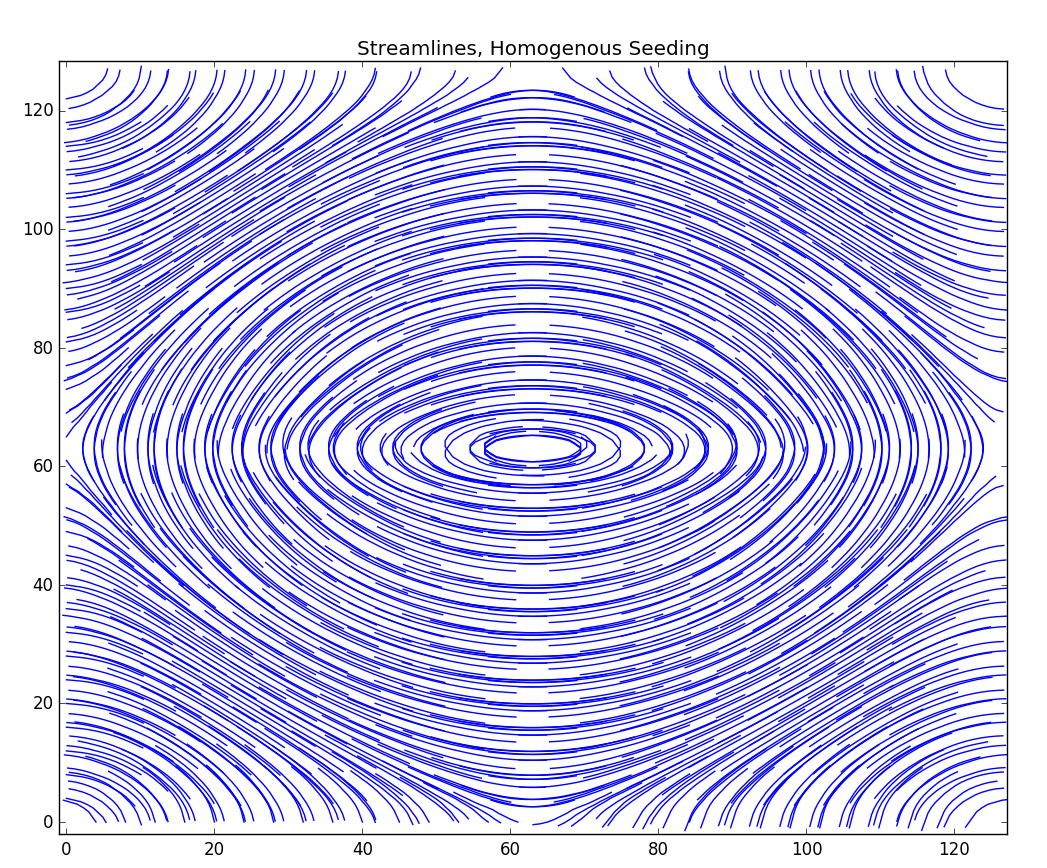
\includegraphics[width=0.55\linewidth]{homo}
 \caption{1000 streamlines integrated with the forward Euler algorithm in the Metsim set. The seeding is homogenously distributed through the vectorfield.}
 \label{fig1}
\end{figure}



\end{document}
